% ============================================================
%  Wind DSM Optimization – PI-PML  |  Capstone Presentation
%  Author : Tapas Barman  (MSD24021)
%  Guide  : Dr. Sirsendu Sekhar Barman
%  Institute: IIIT Lucknow  |  2024-26
%  Slides : 12 (Title + 10 content + Thank You)
% ============================================================
\documentclass[aspectratio=169,10pt]{beamer}

% ─── Theme ───────────────────────────────────────────────────────────────────
\usetheme{metropolis}
\usepackage{appendixnumberbeamer}

% ─── Colour Palette ──────────────────────────────────────────────────────────
\definecolor{IIITblue}{RGB}{0,51,102}
\definecolor{WindBlue}{RGB}{31,119,180}
\definecolor{MLgreen}{RGB}{44,160,44}
\definecolor{DSMred}{RGB}{200,30,30}
\definecolor{MLflow}{RGB}{230,110,20}
\definecolor{LightBg}{RGB}{245,248,252}

\setbeamercolor{frametitle}{bg=IIITblue, fg=white}
\setbeamercolor{progress bar}{fg=MLflow}
\setbeamercolor{title separator}{fg=MLflow}
\setbeamercolor{alerted text}{fg=DSMred}
\setbeamercolor{example text}{fg=MLgreen}
\metroset{block=fill, progressbar=frametitle}

% ─── Packages ────────────────────────────────────────────────────────────────
\usepackage[T1]{fontenc}
\usepackage{lmodern}
\usepackage{amsmath,amssymb}
\usepackage{graphicx}
\usepackage{booktabs}
\usepackage{tabularx}
\usepackage{multirow}
\usepackage{colortbl}
\usepackage{xcolor}
\usepackage{tikz}
\usepackage{pgfplots}
\pgfplotsset{compat=1.18}
\usepackage{fontawesome5}
\usepackage{tcolorbox}
\tcbuselibrary{skins,breakable}
\usepackage{enumitem}

\usetikzlibrary{
  shapes.geometric, shapes.arrows,
  arrows.meta, positioning, fit, calc,
  decorations.pathreplacing, backgrounds,
  patterns
}

% ─── tcolorbox Styles ────────────────────────────────────────────────────────
\tcbset{
  statbox/.style={
    enhanced, colback=IIITblue!7, colframe=IIITblue,
    fonttitle=\bfseries\small, coltitle=white,
    attach boxed title to top left={yshift=-2mm,xshift=4mm},
    boxed title style={colback=IIITblue,rounded corners},
    rounded corners, boxrule=0.6pt, left=4pt, right=4pt, top=4pt, bottom=4pt
  },
  greenbox/.style={
    enhanced, colback=MLgreen!7, colframe=MLgreen!70!black,
    fonttitle=\bfseries\small, coltitle=white,
    attach boxed title to top left={yshift=-2mm,xshift=4mm},
    boxed title style={colback=MLgreen!80!black,rounded corners},
    rounded corners, boxrule=0.6pt, left=4pt, right=4pt, top=4pt, bottom=4pt
  },
  orangebox/.style={
    enhanced, colback=MLflow!8, colframe=MLflow,
    fonttitle=\bfseries\small, coltitle=white,
    attach boxed title to top left={yshift=-2mm,xshift=4mm},
    boxed title style={colback=MLflow,rounded corners},
    rounded corners, boxrule=0.6pt, left=4pt, right=4pt, top=4pt, bottom=4pt
  }
}

% ─── Helpers ─────────────────────────────────────────────────────────────────
\newcommand{\emphblue}[1]{{\color{WindBlue}\textbf{#1}}}
\newcommand{\emphgreen}[1]{{\color{MLgreen}\textbf{#1}}}
\newcommand{\emphred}[1]{{\color{DSMred}\textbf{#1}}}
\newcommand{\emphorange}[1]{{\color{MLflow}\textbf{#1}}}
\newcommand{\rupee}{\textnumero}

% ─── Metadata ────────────────────────────────────────────────────────────────
\title{Wind DSM Optimization}
\subtitle{Physics-Informed Predictive Machine Learning (PI-PML)}
\author{Tapas Barman \\ \small MSD24021}
\institute{%
  \textbf{Supervisor:} Dr.\ Sirsendu Sekhar Barman \\[2pt]
  Department of Mathematics,
  Indian Institute of Information Technology, Lucknow
}
\date{May 2026}

%=============================================================================
\begin{document}
%=============================================================================

%────────────────────────────────────────────────────────────────────────────
% SLIDE 1 — TITLE
%────────────────────────────────────────────────────────────────────────────
{
\setbeamercolor{background canvas}{bg=IIITblue}
\begin{frame}[plain]
  \vspace{0.5cm}
  \begin{columns}[c]
    \column{0.75\textwidth}
      {\color{white}\LARGE\bfseries Wind DSM Optimization}\\[5pt]
      {\color{MLflow}\large Physics-Informed Predictive Machine Learning (PI-PML)}\\[16pt]
      {\color{white!85}\normalsize Tapas Barman \quad|\quad MSD24021}\\[3pt]
      {\color{white!65}\small Supervisor: Dr.\ Sirsendu Sekhar Barman}\\[2pt]
      {\color{white!55}\small Dept.\ of Mathematics, IIIT Lucknow}\\[8pt]
      {\color{white!45}\footnotesize MSc.\ Data Science $\cdot$ 2024--26}
    \column{0.22\textwidth}
      \centering
      
\includegraphics[width=\textwidth]{../iiitl_logo.png}
  \end{columns}
  \vfill
  {\color{white!30}\rule{\textwidth}{0.4pt}}\\[2pt]
  {\color{white!30}\tiny May 2026 \hfill IIIT Lucknow}
\end{frame}
}

%────────────────────────────────────────────────────────────────────────────
% SLIDE 2 — BACKGROUND & PROBLEM
%────────────────────────────────────────────────────────────────────────────
\begin{frame}{Background \& Problem Statement}
  \begin{columns}[T]
    \column{0.50\textwidth}
      \begin{tcolorbox}[statbox, title={\faIndustry\; CERC DSM Framework}]
        \begin{itemize}[leftmargin=1em, itemsep=4pt, font=\small]
          \item Every generator submits a \emphblue{day-ahead 96-block} schedule (15-min intervals)
          \item Deviations attract \emphred{tiered financial penalties}
          \item Wind is \emphred{stochastic} — even 15–20\% hub-height error triggers the highest penalty slab (\emphred{\rupee{}1.50/unit})
        \end{itemize}
      \end{tcolorbox}

      \vspace{6pt}
      \begin{block}{Research Question}
        \small\textit{How can operators reduce CERC DSM liability through more accurate 96-block forecasts, combining physics-based turbine modelling with ML?}
      \end{block}

    \column{0.47\textwidth}
      \centering
      \small\textbf{CERC DSM Penalty Escalation}\\[4pt]
      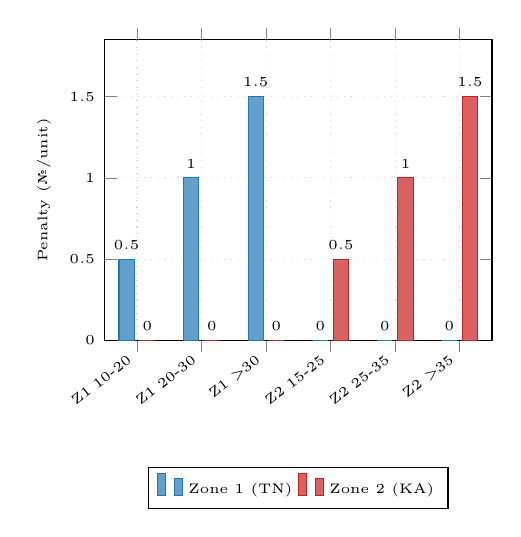
\begin{tikzpicture}
        \begin{axis}[
          ybar, bar width=5.5pt,
          width=6.5cm, height=5.4cm,
          symbolic x coords={Z1 10-20, Z1 20-30, Z1 {>}30, Z2 15-25, Z2 25-35, Z2 {>}35},
          xtick=data,
          x tick label style={rotate=38, anchor=east, font=\tiny},
          ymin=0, ymax=1.85,
          ylabel={\tiny Penalty (\rupee/unit)},
          ylabel style={font=\tiny},
          nodes near coords,
          nodes near coords style={font=\tiny},
          grid=major, grid style={dotted,gray!30},
          tick label style={font=\tiny},
          legend style={at={(0.5,-0.42)}, anchor=north, font=\tiny, legend columns=2},
        ]
          \addplot[fill=WindBlue!70, draw=WindBlue]
            coordinates {(Z1 10-20,0.5)(Z1 20-30,1.0)(Z1 {>}30,1.5)
                         (Z2 15-25,0)(Z2 25-35,0)(Z2 {>}35,0)};
          \addplot[fill=DSMred!70, draw=DSMred]
            coordinates {(Z1 10-20,0)(Z1 20-30,0)(Z1 {>}30,0)
                         (Z2 15-25,0.5)(Z2 25-35,1.0)(Z2 {>}35,1.5)};
          \legend{Zone 1 (TN), Zone 2 (KA)}
        \end{axis}
      \end{tikzpicture}
  \end{columns}
\end{frame}

%────────────────────────────────────────────────────────────────────────────
% SLIDE 3 — SYSTEM ARCHITECTURE
%────────────────────────────────────────────────────────────────────────────
\begin{frame}{System Architecture — Full PI-PML Pipeline}
  \centering
  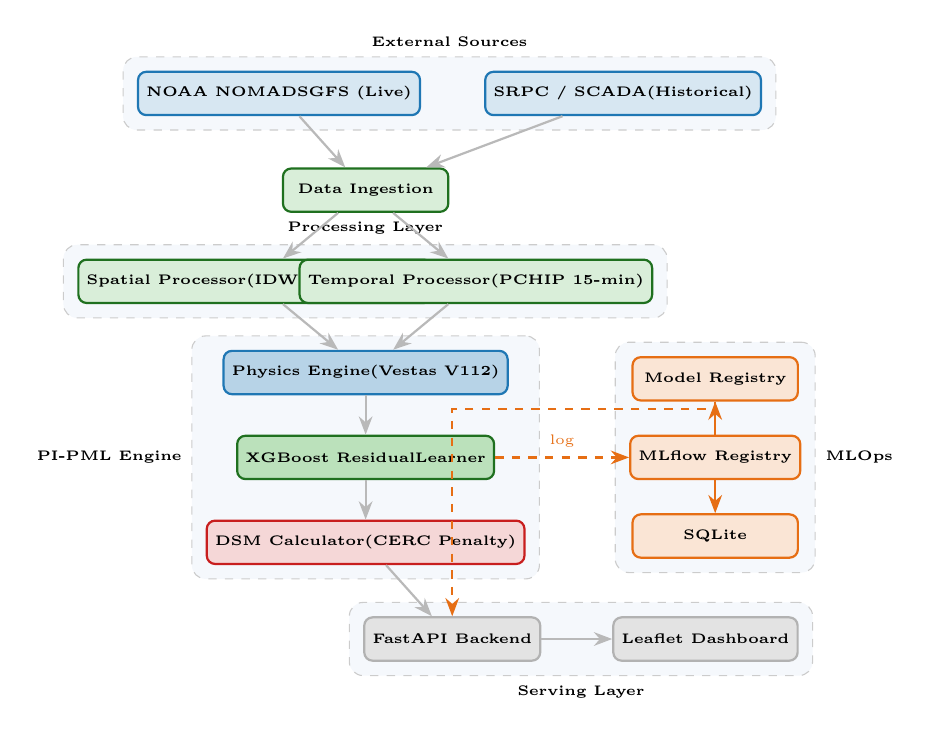
\begin{tikzpicture}[
    node distance=0.42cm and 0.75cm,
    box/.style={rectangle, rounded corners=3pt, draw, thick,
                minimum width=2.1cm, minimum height=0.55cm,
                font=\tiny\bfseries, text centered, inner sep=3pt},
    srcbox/.style={box, fill=WindBlue!18, draw=WindBlue},
    procbox/.style={box, fill=MLgreen!18, draw=MLgreen!70!black},
    engbox/.style={box, fill=WindBlue!32, draw=WindBlue},
    mlbox/.style={box, fill=MLgreen!32, draw=MLgreen!70!black},
    dsmbox/.style={box, fill=DSMred!18, draw=DSMred},
    storebox/.style={box, fill=MLflow!18, draw=MLflow},
    servebox/.style={box, fill=gray!22, draw=gray!60},
    arr/.style={-Stealth, thick, gray!55},
    grp/.style={draw=gray!40, dashed, rounded corners=5pt, fill=LightBg, inner sep=5pt}
  ]
    \node[srcbox] (noaa) {NOAA NOMADS\\GFS (Live)};
    \node[srcbox, right=0.8cm of noaa] (srpc) {SRPC / SCADA\\(Historical)};
    \node[procbox, below=0.65cm of noaa, xshift=1.1cm] (di) {Data Ingestion};
    \node[procbox, below=0.58cm of di, xshift=-1.4cm] (sp) {Spatial Processor\\(IDW+Log-Profile)};
    \node[procbox, below=0.58cm of di, xshift=1.4cm]  (tp) {Temporal Processor\\(PCHIP 15-min)};
    \node[engbox, below=0.58cm of sp, xshift=1.4cm] (pe) {Physics Engine\\(Vestas V112)};
    \node[mlbox,  below=0.5cm of pe]  (ml) {XGBoost Residual\\Learner};
    \node[dsmbox, below=0.5cm of ml]  (dsm){DSM Calculator\\(CERC Penalty)};
    \node[storebox, right=1.7cm of ml]  (mlf) {MLflow Registry};
    \node[storebox, below=0.42cm of mlf] (db)  {SQLite};
    \node[storebox, above=0.42cm of mlf] (reg) {Model Registry};
    \node[servebox, below=0.65cm of dsm, xshift=1.1cm] (api) {FastAPI Backend};
    \node[servebox, right=0.9cm of api] (ui)  {Leaflet Dashboard};

    \draw[arr](noaa)--(di); \draw[arr](srpc)--(di);
    \draw[arr](di)--(sp);   \draw[arr](di)--(tp);
    \draw[arr](sp)--(pe);   \draw[arr](tp)--(pe);
    \draw[arr](pe)--(ml);   \draw[arr](ml)--(dsm);
    \draw[arr](dsm)--(api); \draw[arr](api)--(ui);
    \draw[arr,dashed,MLflow](ml) -- node[above,font=\tiny,text=MLflow]{log} (mlf);
    \draw[arr,MLflow](mlf)--(db); \draw[arr,MLflow](mlf)--(reg);
    \draw[arr,dashed,MLflow](reg)--++(0,-0.38)-|(api);

    \begin{scope}[on background layer]
      \node[grp,fit=(noaa)(srpc),label={[font=\tiny\bfseries]above:External Sources}]{};
      \node[grp,fit=(sp)(tp),label={[font=\tiny\bfseries]above:Processing Layer}]{};
      \node[grp,fit=(pe)(ml)(dsm),label={[font=\tiny\bfseries]left:PI-PML Engine}]{};
      \node[grp,fit=(mlf)(db)(reg),label={[font=\tiny\bfseries]right:MLOps}]{};
      \node[grp,fit=(api)(ui),label={[font=\tiny\bfseries]below:Serving Layer}]{};
    \end{scope}
  \end{tikzpicture}
\end{frame}

%────────────────────────────────────────────────────────────────────────────
% SLIDE 4 — DOUBLE-ENGINE DESIGN
%────────────────────────────────────────────────────────────────────────────
\begin{frame}{The Double-Engine PI-PML Design}
  \begin{columns}[T]
    \column{0.50\textwidth}
      \begin{tcolorbox}[statbox, title={\faAtom\; Core Concept}]
        \begin{enumerate}[leftmargin=1.2em, itemsep=5pt, font=\small]
          \item \emphblue{Engine 1 — Physics Baseline}: Deterministic turbine output via \texttt{windpowerlib} (Vestas V112, hub height 84~m)
          \item \emphgreen{Engine 2 — XGBoost Residual}: Predicts the \textit{signed error} of the physics model
        \end{enumerate}
      \end{tcolorbox}

      \vspace{6pt}
      \begin{block}{Final Forecast Equation}
        \[
          \hat{P}_{\text{final}}(t) =
          \underbrace{P_{\text{physics}}(t)}_{\text{Engine 1}} +
          \underbrace{\hat{\varepsilon}_{\text{XGB}}(t)}_{\text{Engine 2}}
        \]
      \end{block}

      \vspace{6pt}
      \textbf{Key physics enhancements:}
      \begin{itemize}[leftmargin=1em, itemsep=3pt, font=\small]
        \item \emphblue{Moist air density} via Tetens equation (monsoon correction)
        \item \emphblue{Log-profile hub-height} wind scaling ($z_r \rightarrow 84$~m)
        \item \emphblue{Elevation speedup} for Deccan Plateau terrain
        \item \emphblue{DFIG efficiency losses} at low wind speeds
      \end{itemize}

    \column{0.47\textwidth}
      \centering
      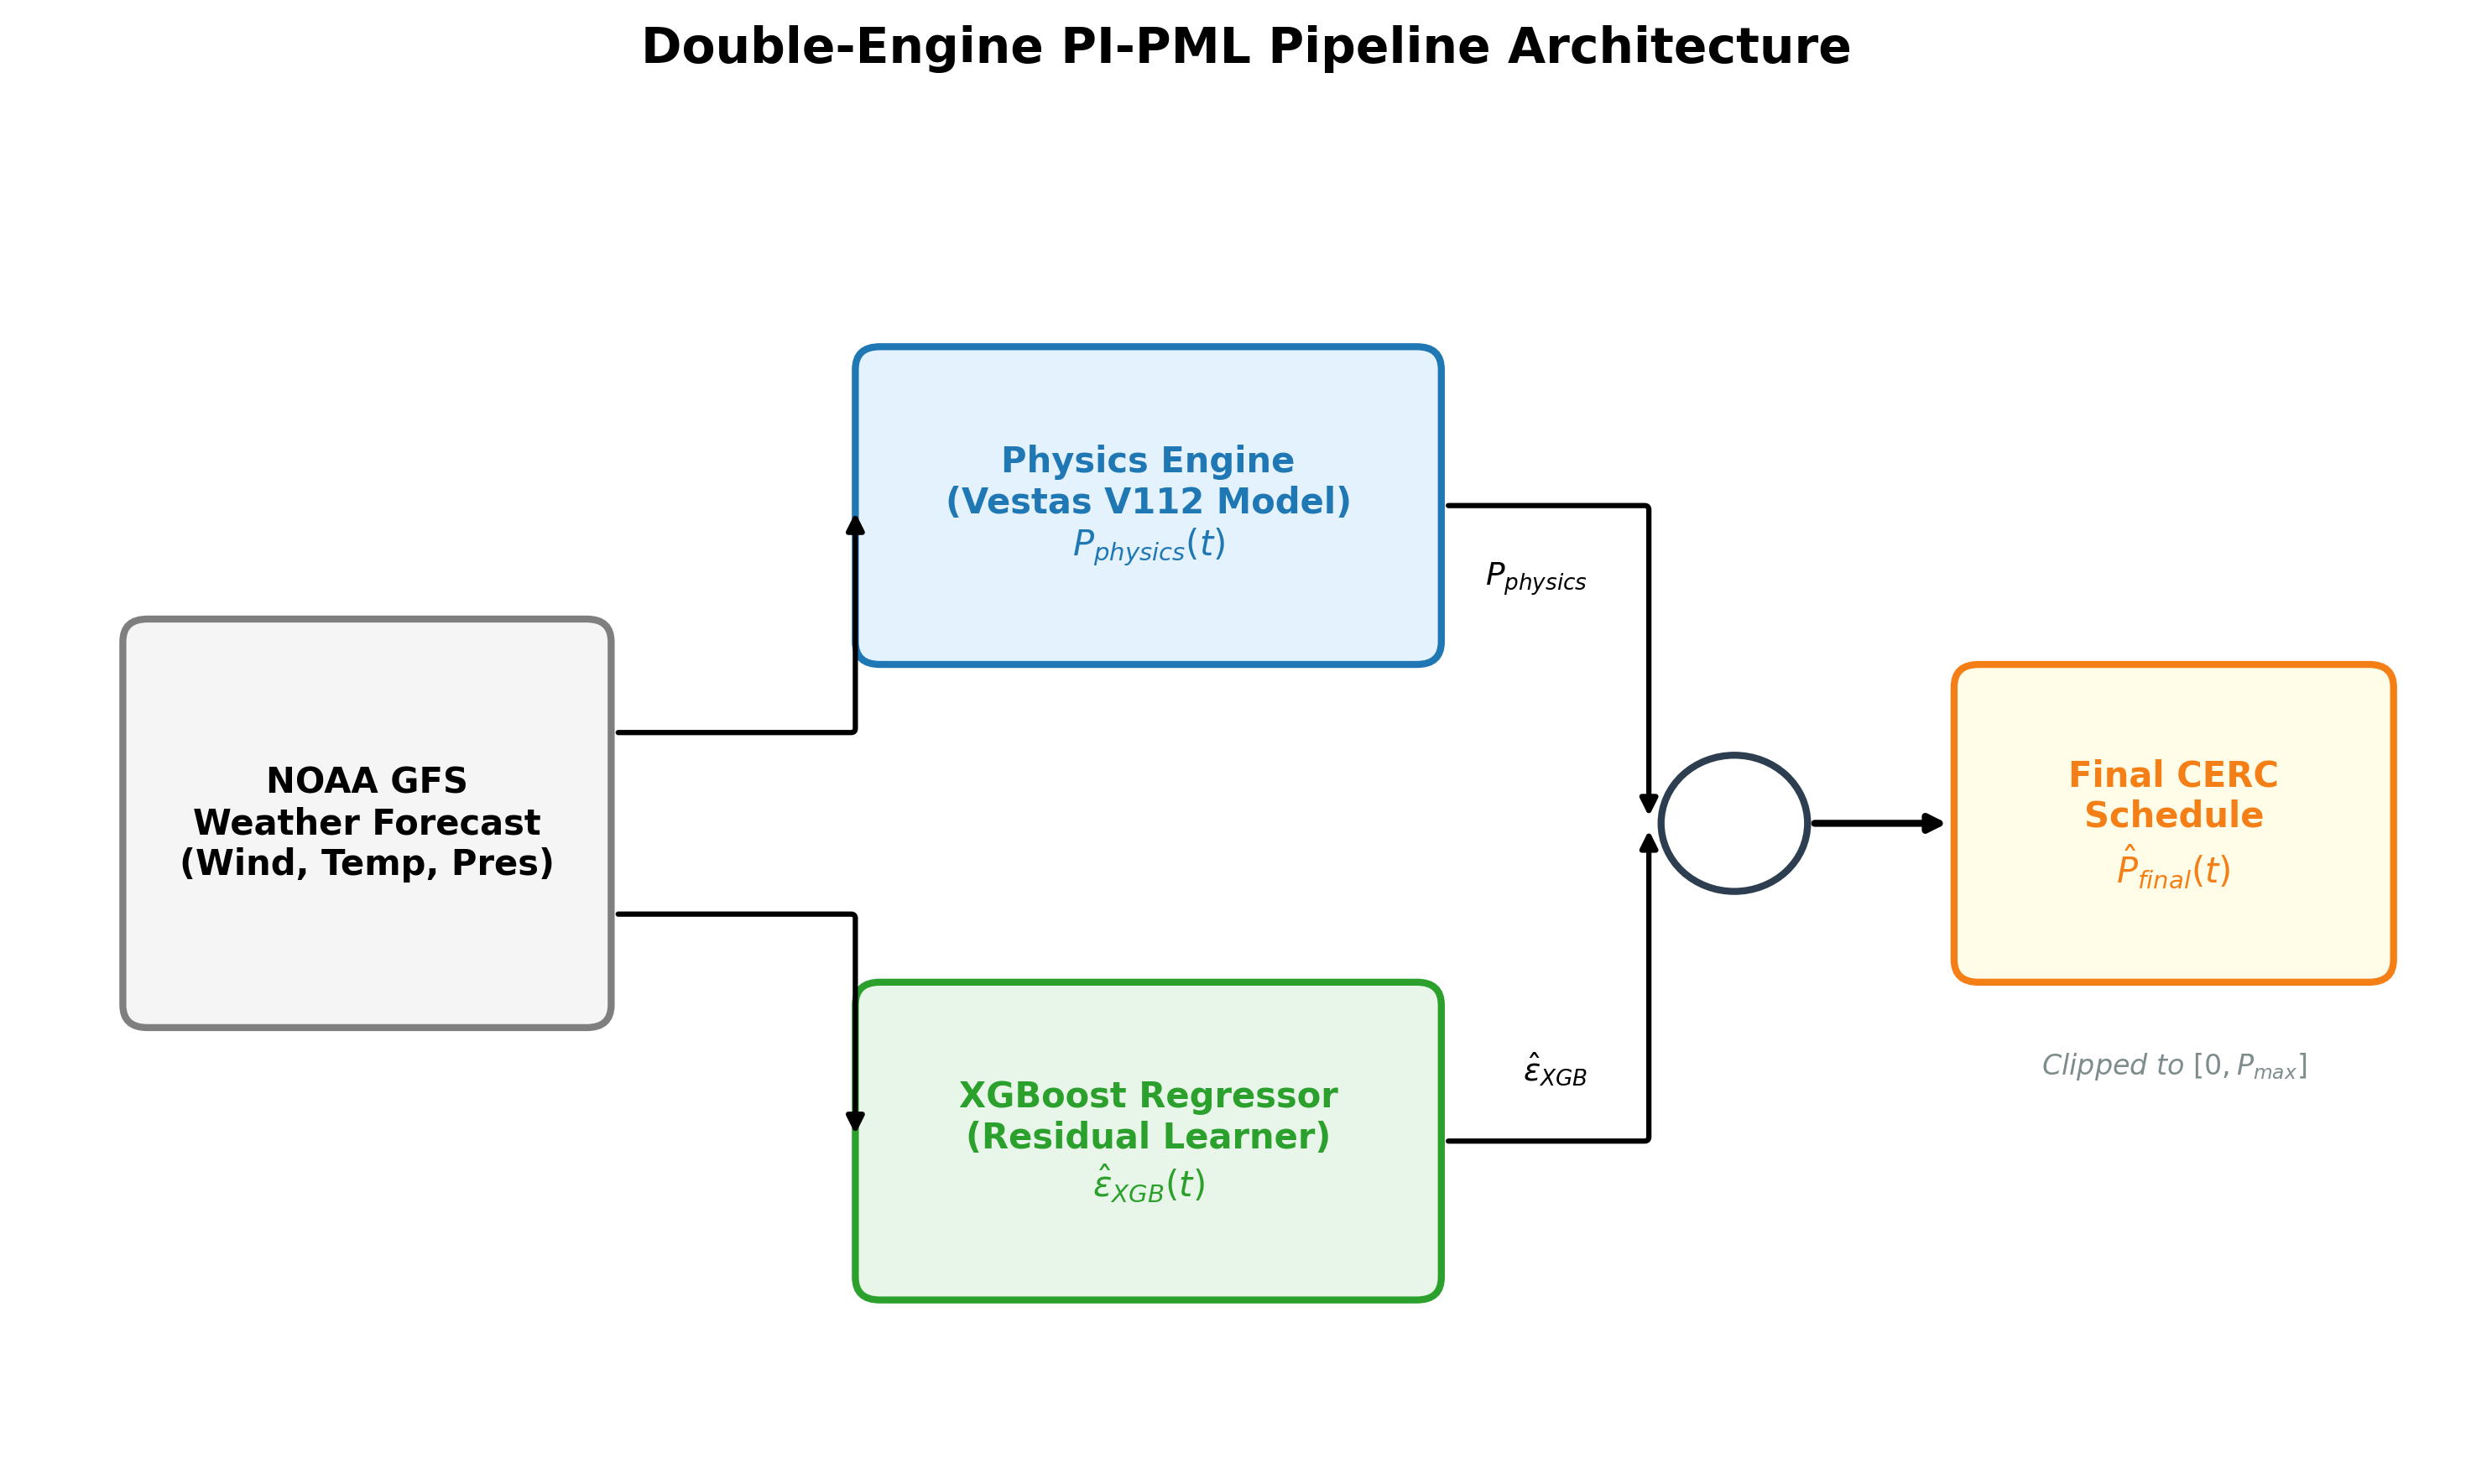
\includegraphics[width=\textwidth]{../double_engine_diagram.png}
      \\[5pt]
      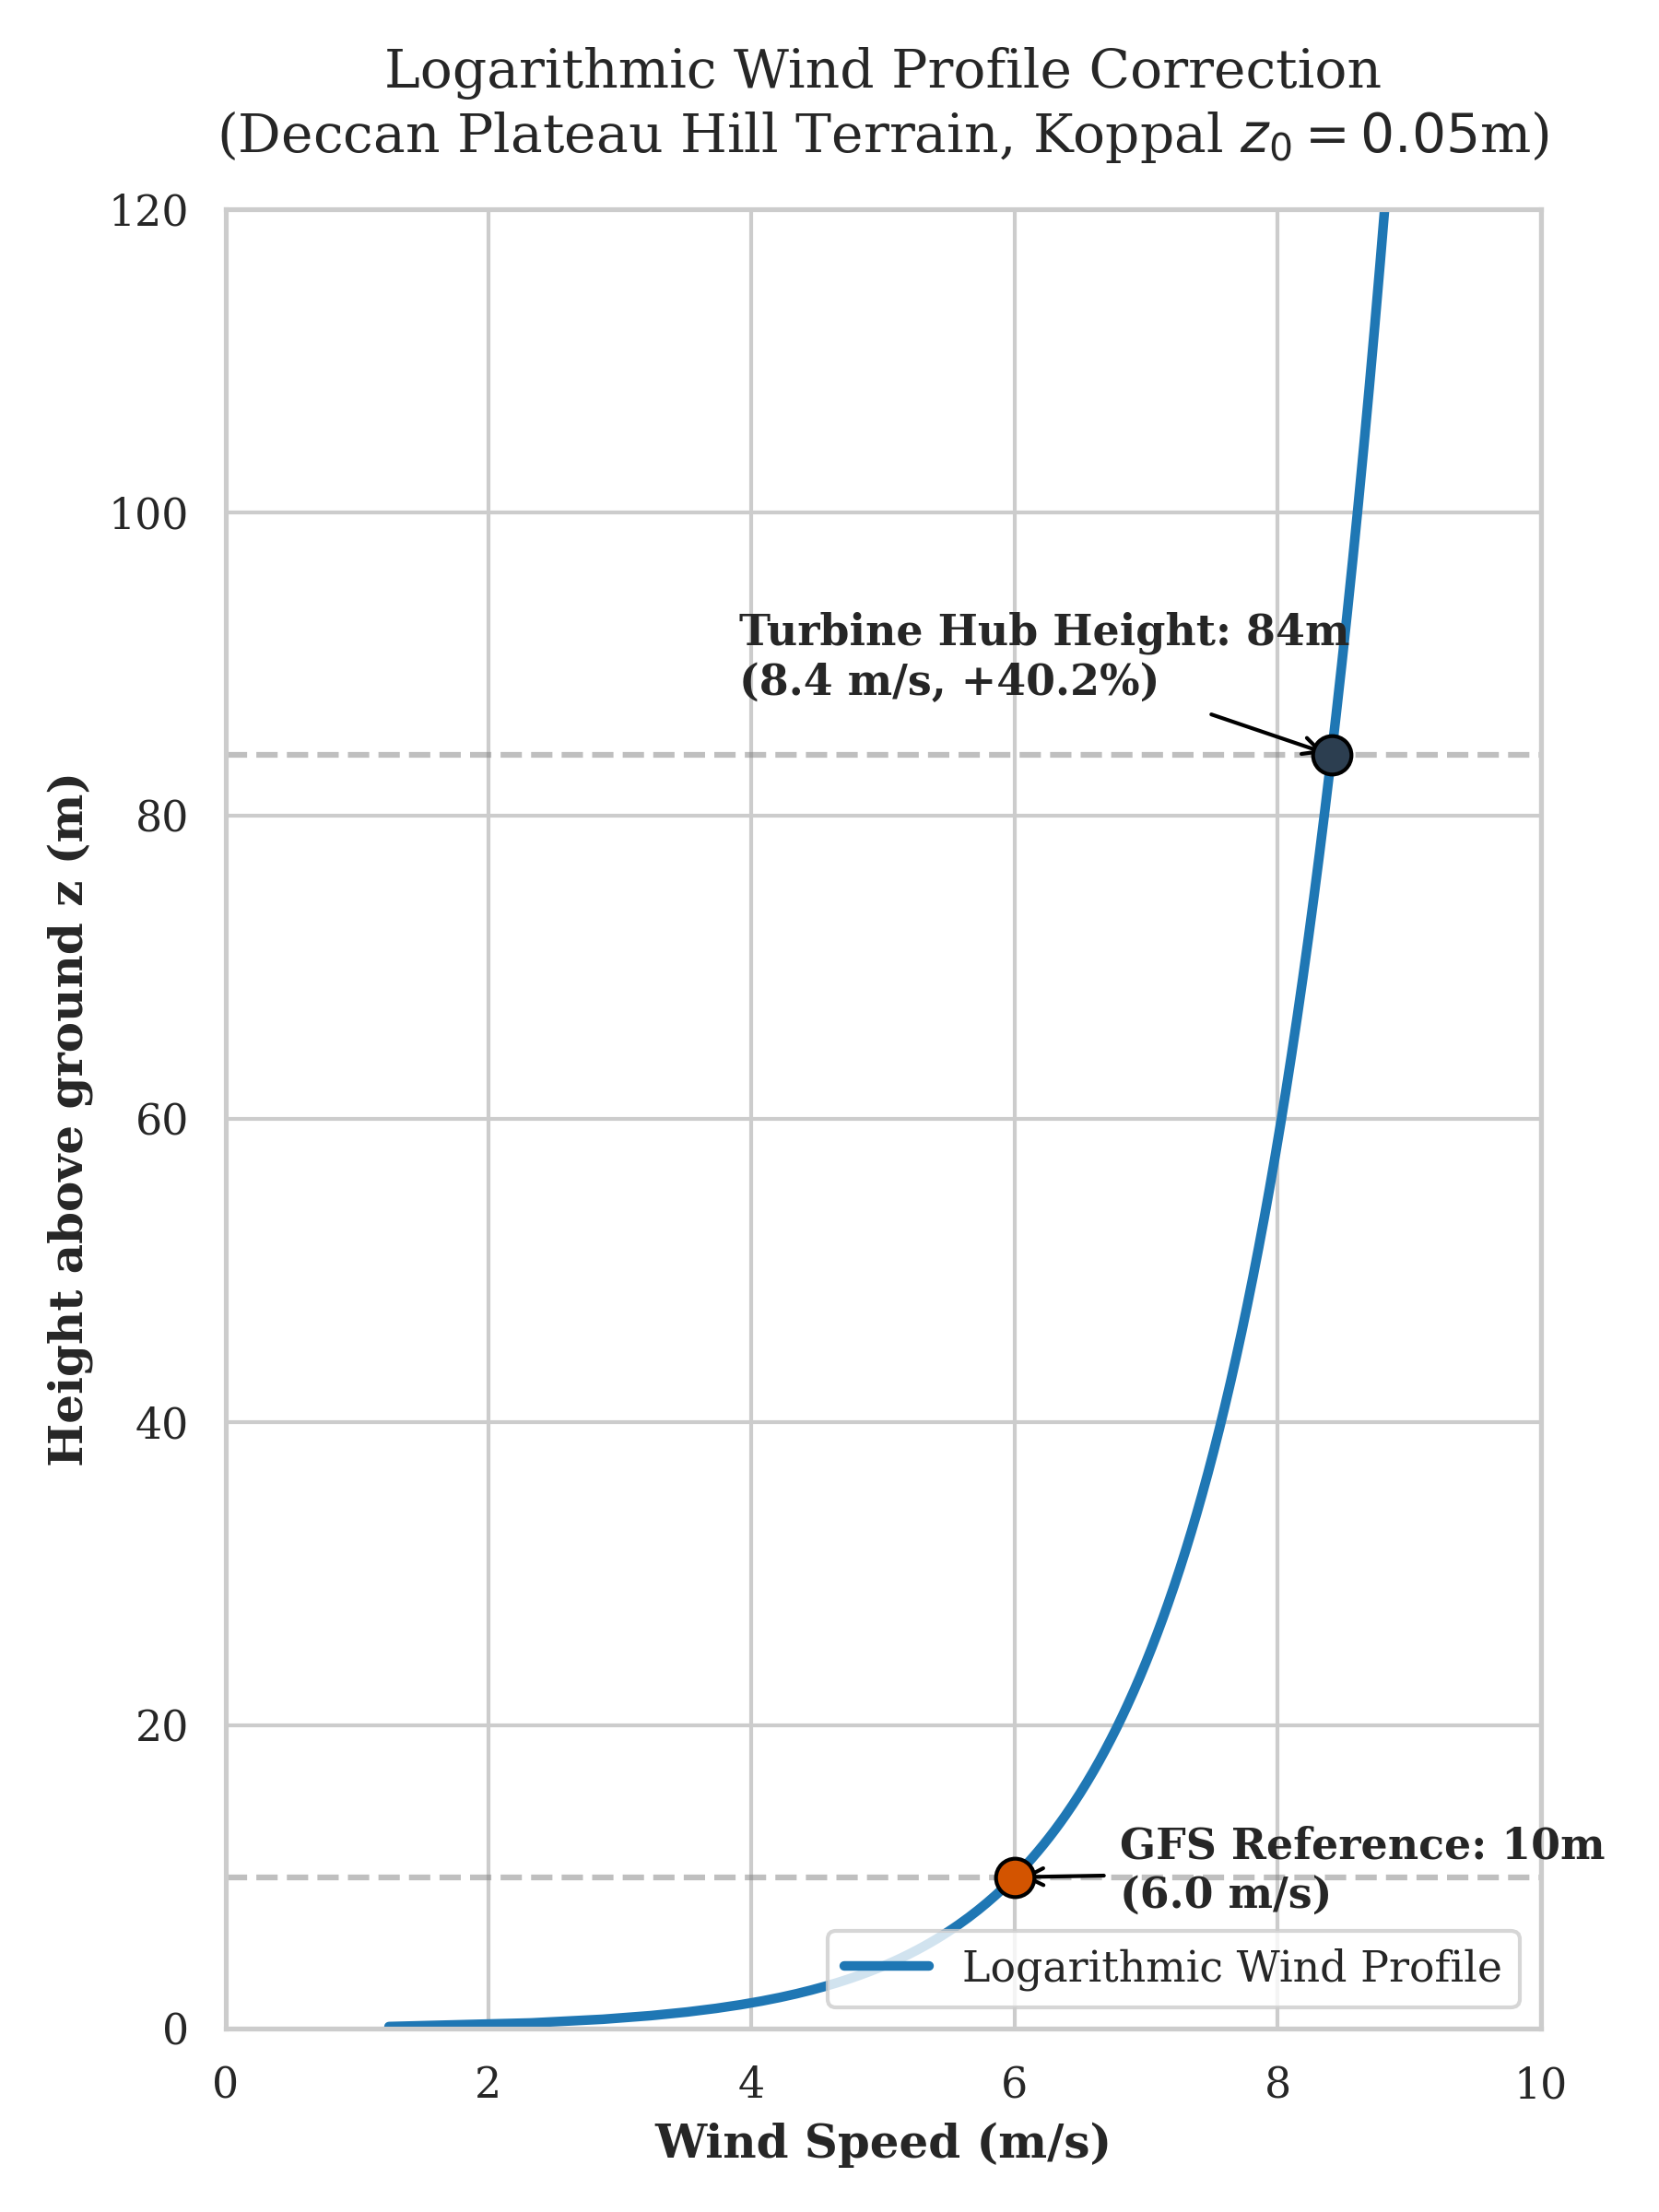
\includegraphics[width=\textwidth]{../log_profile.png}
      \\[2pt]
      \tiny Log-profile correction: hub-height wind is \textbf{31\% higher} than the 10~m GFS reference.
  \end{columns}
\end{frame}

%────────────────────────────────────────────────────────────────────────────
% SLIDE 5 — DATA PIPELINE (SPATIAL + TEMPORAL)
%────────────────────────────────────────────────────────────────────────────
\begin{frame}{Data Pipeline — Downscaling \& Interpolation}
  \begin{columns}[T]
    \column{0.49\textwidth}
      \begin{tcolorbox}[statbox, title={\faGlobe\; Spatial Downscaling (25~km $\to$ 1~km)}]
        \begin{itemize}[leftmargin=1em, itemsep=4pt, font=\small]
          \item Live GFS fetched async from \emphblue{NOAA NOMADS} every 6 hrs
          \item \emphblue{Bilinear spline} maps grid to exact plant coordinate
          \item \emphblue{Logarithmic wind profile} scales to hub height $z_h$:
            \[ u(z_h)=u(z_r)\cdot\frac{\ln(z_h/z_0)}{\ln(z_r/z_0)} \]
          \item Roughness $z_0$ and elevation speedup applied
        \end{itemize}
      \end{tcolorbox}

    \column{0.49\textwidth}
      \begin{tcolorbox}[orangebox, title={\faClock\; Temporal Interpolation (3-hr $\to$ 15-min)}]
        \begin{itemize}[leftmargin=1em, itemsep=4pt, font=\small]
          \item GFS provides \emphred{8 points/day}; CERC requires \emphblue{96 blocks/day}
          \item \emphblue{PCHIP} interpolation (Piecewise Cubic Hermite) guarantees:
            \begin{itemize}[leftmargin=1em, itemsep=2pt]
              \item \emphgreen{Monotonicity} — no non-physical overshoots
              \item Smooth wind ramp tracking
            \end{itemize}
        \end{itemize}
      \end{tcolorbox}

      \vspace{6pt}
      \begin{tcolorbox}[greenbox, title={\faBrain\; XGBoost Feature Groups}]
        \begin{tabular}{@{}ll@{}}
          \tiny\textbf{Group} & \tiny\textbf{Examples} \\
          \midrule
          \tiny Physics output & \tiny $P_\text{phys}$, $u_{z_h}$, $\rho_\text{moist}$ \\
          \tiny Atmospheric & \tiny $T_2$, RH, $p_s$, $\theta_\text{wind}$ \\
          \tiny Temporal & \tiny Block \#, hour, day-of-year \\
          \tiny Terrain & \tiny $z_0$, elevation, speedup $S$ \\
          \tiny Lagged residuals & \tiny $\varepsilon(t{-}1)$, $\varepsilon(t{-}2)$, $\varepsilon(t{-}4)$ \\
        \end{tabular}
      \end{tcolorbox}
  \end{columns}
\end{frame}

%────────────────────────────────────────────────────────────────────────────
% SLIDE 6 — DSM CALCULATOR
%────────────────────────────────────────────────────────────────────────────
\begin{frame}{CERC DSM Calculator — 3 Regulatory Zones}
  \begin{center}
    \renewcommand{\arraystretch}{1.45}
    \small
    \begin{tabularx}{\textwidth}{@{}lXXX@{}}
      \toprule
      \textbf{Zone} & \textbf{Tolerance} & \textbf{Denominator} & \textbf{Penalty Slabs} \\
      \midrule
      \rowcolor{WindBlue!10}
      \textbf{Zone 1} \small(Tight — TN) & 10\% & Available Capacity &
        10–20\%: \rupee{}0.50/u \newline 20–30\%: \rupee{}1.00/u \newline $>$30\%: \rupee{}1.50/u \\[2pt]
      \rowcolor{MLgreen!10}
      \textbf{Zone 2} \small(Standard — KA) & 15\% & Available Capacity &
        15–25\%: \rupee{}0.50/u \newline 25–35\%: \rupee{}1.00/u \newline $>$35\%: \rupee{}1.50/u \\[2pt]
      \rowcolor{MLflow!10}
      \textbf{Zone 3} \small(Market — Khavda) & 10\% & Sched.\ Generation &
        $>$10\%: 10\% of PPA Rate/unit \\
      \bottomrule
    \end{tabularx}
  \end{center}

  \vspace{4pt}
  \begin{columns}[T]
    \column{0.48\textwidth}
      \begin{tcolorbox}[statbox, title={\faClock\; Dynamic ACP Multipliers}]
        \begin{tabular}{@{}lll@{}}
          \small\textbf{Period} & \small\textbf{Time} & \small\textbf{Mult.} \\
          \midrule
          \small Morning Peak  & \small 06--09h & \small\emphred{1.5×} \\
          \small Evening Peak  & \small 18--22h & \small\emphred{2.5×} \\
          \small Night Off-Peak& \small 00--05h & \small 0.8× \\
          \small Normal        & \small Other   & \small 1.0× \\
        \end{tabular}
      \end{tcolorbox}
    \column{0.48\textwidth}
      \begin{alertblock}{RSOPL Koppal — Zone 2}
        Karnataka operates under \emphred{Zone 2 (Standard)} rules. The PI-PML system is validated specifically under this regulatory regime with a \textbf{15\% free tolerance band}.
      \end{alertblock}
  \end{columns}
\end{frame}

%────────────────────────────────────────────────────────────────────────────
% SLIDE 7 — MLOPS: CHAMPION-CHALLENGER
%────────────────────────────────────────────────────────────────────────────
\begin{frame}{MLOps — Champion-Challenger Framework}
  \begin{columns}[T]
    \column{0.48\textwidth}
      \begin{tcolorbox}[orangebox, title={\faExchangeAlt\; Promotion Logic}]
        \begin{enumerate}[leftmargin=1.2em, itemsep=5pt, font=\small]
          \item Upload new \emphblue{SCADA CSV}
          \item Train \emphgreen{Challenger} on 80\% chronological split
          \item Evaluate both Champion \& Challenger on 20\% hold-out
          \item \textbf{Promote only if} Challenger \emphred{CERC penalty} $<$ Champion
          \item \emphgreen{Zero-downtime} — API resolves model URI dynamically
        \end{enumerate}
      \end{tcolorbox}

      \vspace{6pt}
      \begin{block}{MLflow Model URI}
        \small\ttfamily models:/Wind\_DSM\_Residual\_\{park\_id\}/Production
      \end{block}

      \vspace{4pt}
      \begin{alertblock}{Key Design Choice}
        Promotion criterion is \emphred{CERC penalty}, not raw MAE — aligning the ML objective with real financial risk.
      \end{alertblock}

    \column{0.48\textwidth}
      \centering
      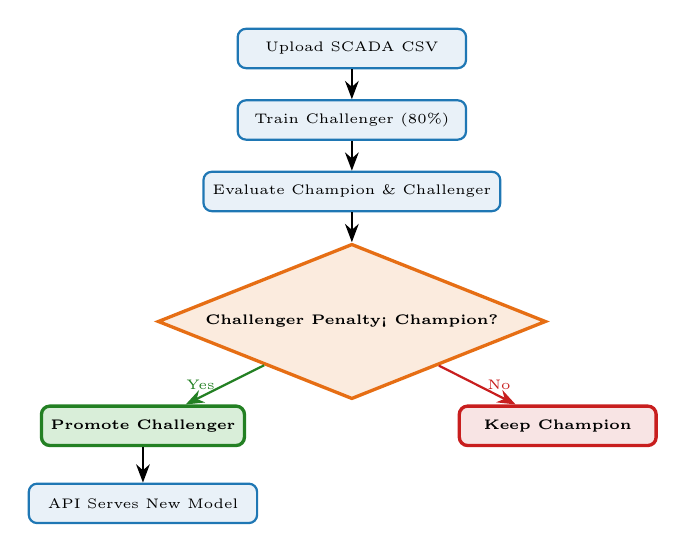
\begin{tikzpicture}[
        node distance=0.38cm and 0.9cm,
        proc/.style={rectangle,rounded corners=3pt,draw=WindBlue,thick,
                     fill=WindBlue!10,minimum width=2.9cm,minimum height=0.5cm,
                     font=\tiny,text centered},
        dec/.style={diamond,draw=MLflow,very thick,fill=MLflow!14,
                    minimum width=2.6cm,minimum height=0.5cm,
                    font=\tiny\bfseries,text centered,aspect=2.5},
        good/.style={rectangle,rounded corners=3pt,draw=MLgreen!80!black,very thick,
                     fill=MLgreen!18,minimum width=2.5cm,minimum height=0.5cm,
                     font=\tiny\bfseries,text centered},
        bad/.style={rectangle,rounded corners=3pt,draw=DSMred,very thick,
                    fill=DSMred!12,minimum width=2.5cm,minimum height=0.5cm,
                    font=\tiny\bfseries,text centered},
        arr/.style={-Stealth,thick}
      ]
        \node[proc] (upload){Upload SCADA CSV};
        \node[proc,below=of upload](train){Train Challenger (80\%)};
        \node[proc,below=of train](eval){Evaluate Champion \& Challenger};
        \node[dec, below=of eval](decide){Challenger Penalty\\< Champion?};
        \node[good,below left=0.55cm and 0.1cm of decide](promote){Promote Challenger};
        \node[bad, below right=0.55cm and 0.1cm of decide](keep){Keep Champion};
        \node[proc,below=0.45cm of promote](serve){API Serves New Model};

        \draw[arr](upload)--(train); \draw[arr](train)--(eval); \draw[arr](eval)--(decide);
        \draw[arr,MLgreen!80!black](decide)--node[left,font=\tiny]{Yes}(promote);
        \draw[arr,DSMred](decide)--node[right,font=\tiny]{No}(keep);
        \draw[arr](promote)--(serve);
      \end{tikzpicture}
  \end{columns}
\end{frame}

%────────────────────────────────────────────────────────────────────────────
% SLIDE 8 — WEB DASHBOARD
%────────────────────────────────────────────────────────────────────────────
\begin{frame}{Interactive Web Dashboard \& API}
  \begin{columns}[T]
    \column{0.52\textwidth}
      \textbf{Dashboard Features:}
      \begin{itemize}[leftmargin=1.2em, itemsep=5pt, font=\small]
        \item \faMap\; \emphblue{Leaflet Interactive Map} — Indian wind park clusters with geographical overlays
        \item \faWind\; \emphblue{Animated Wind Vectors} — live direction \& speed from Open-Meteo GFS
        \item \faPalette\; \emphblue{Neon Themes} — Midnight Cyan, Neon Purple, Emerald Green, Golden Amber
        \item \faTerminal\; \emphblue{Operator Command Centre:}
          \begin{itemize}[leftmargin=1em, itemsep=2pt, font=\small]
            \item Fetch live 96-block GFS forecast
            \item Upload SCADA CSV $\to$ trigger retrain
            \item Toggle Pre-Trained / Custom model
            \item Download CERC-compliant 96-block CSV
          \end{itemize}
        \item \faDocker\; \emphblue{Docker deployment} via \texttt{docker-compose up -{}-build}
      \end{itemize}

    \column{0.45\textwidth}
      \begin{tcolorbox}[statbox, title={\faPlug\; FastAPI Endpoints}]
        \ttfamily\scriptsize
        \begin{tabular}{@{}ll@{}}
          \textcolor{MLgreen}{POST} & /api/v1/forecast/\{park\_id\} \\
          \textcolor{MLgreen}{POST} & /api/v1/retrain/\{park\_id\} \\
          \textcolor{WindBlue}{GET}  & /api/v1/job-status/\{job\_id\} \\
          \textcolor{WindBlue}{GET}  & /api/v1/download-forecast/ \\
                & \quad\{park\_id\} \\
          \textcolor{WindBlue}{GET}  & /api/v1/wind-vectors \\
          \textcolor{WindBlue}{GET}  & /api/v1/custom-model-exists/ \\
                & \quad\{park\_id\} \\
        \end{tabular}
      \end{tcolorbox}

      \vspace{6pt}
      \begin{tcolorbox}[greenbox, title={\faCogs\; Tech Stack}]
        \begin{itemize}[leftmargin=1em, itemsep=2pt, font=\scriptsize]
          \item windpowerlib, XGBoost, MLflow
          \item FastAPI + Uvicorn
          \item Leaflet.js, NOAA NOMADS GFS
          \item Docker + SQLite
        \end{itemize}
      \end{tcolorbox}
  \end{columns}
\end{frame}

%────────────────────────────────────────────────────────────────────────────
% SLIDE 9 — RESULTS
%────────────────────────────────────────────────────────────────────────────
\begin{frame}{Experimental Results — RSOPL Koppal (75~MW)}
  \begin{columns}[T]
    \column{0.50\textwidth}
      \textbf{Validation Dataset:}
      \begin{itemize}[leftmargin=1em, itemsep=3pt, font=\small]
        \item \emphblue{29,568 official SRPC blocks} — 10 continuous months
        \item Location: Koppal, Karnataka (Zone 2)
        \item Turbine: Vestas V112-3.0~MW $\times$ 25
        \item Train: 8 months (80\%) | Test: 2 months (20\%)
      \end{itemize}

      \vspace{8pt}
      \begin{center}
        \renewcommand{\arraystretch}{1.45}
        \small
        \begin{tabular}{@{}lcc@{}}
          \toprule
          \textbf{Metric} & \textbf{Physics} & \textbf{PI-PML} \\
          \midrule
          \rowcolor{gray!8}
          MAE Reduction & --- & \emphgreen{\textbf{71.2\%}} \\
          CERC Penalty & \emphred{\rupee{}24,83,254} & \emphgreen{\rupee{}1,29,282} \\
          \rowcolor{gray!8}
          Net Savings & \multicolumn{2}{c}{\emphgreen{\textbf{\rupee{}23.5~Lakhs}}} \\
          Annual Proj. & \multicolumn{2}{c}{\emphgreen{\textbf{\rupee{}1.41~Crores/yr}}} \\
          \bottomrule
        \end{tabular}
      \end{center}

      \vspace{6pt}
      \begin{tcolorbox}[greenbox, title={Penalty Reduction}]
        \centering\small
        \emphred{\rupee{}24.8 Lakhs} $\longrightarrow$ \emphgreen{\rupee{}1.3 Lakhs}\\[2pt]
        \textbf{94.8\% penalty reduction}
      \end{tcolorbox}

    \column{0.47\textwidth}
      \centering
      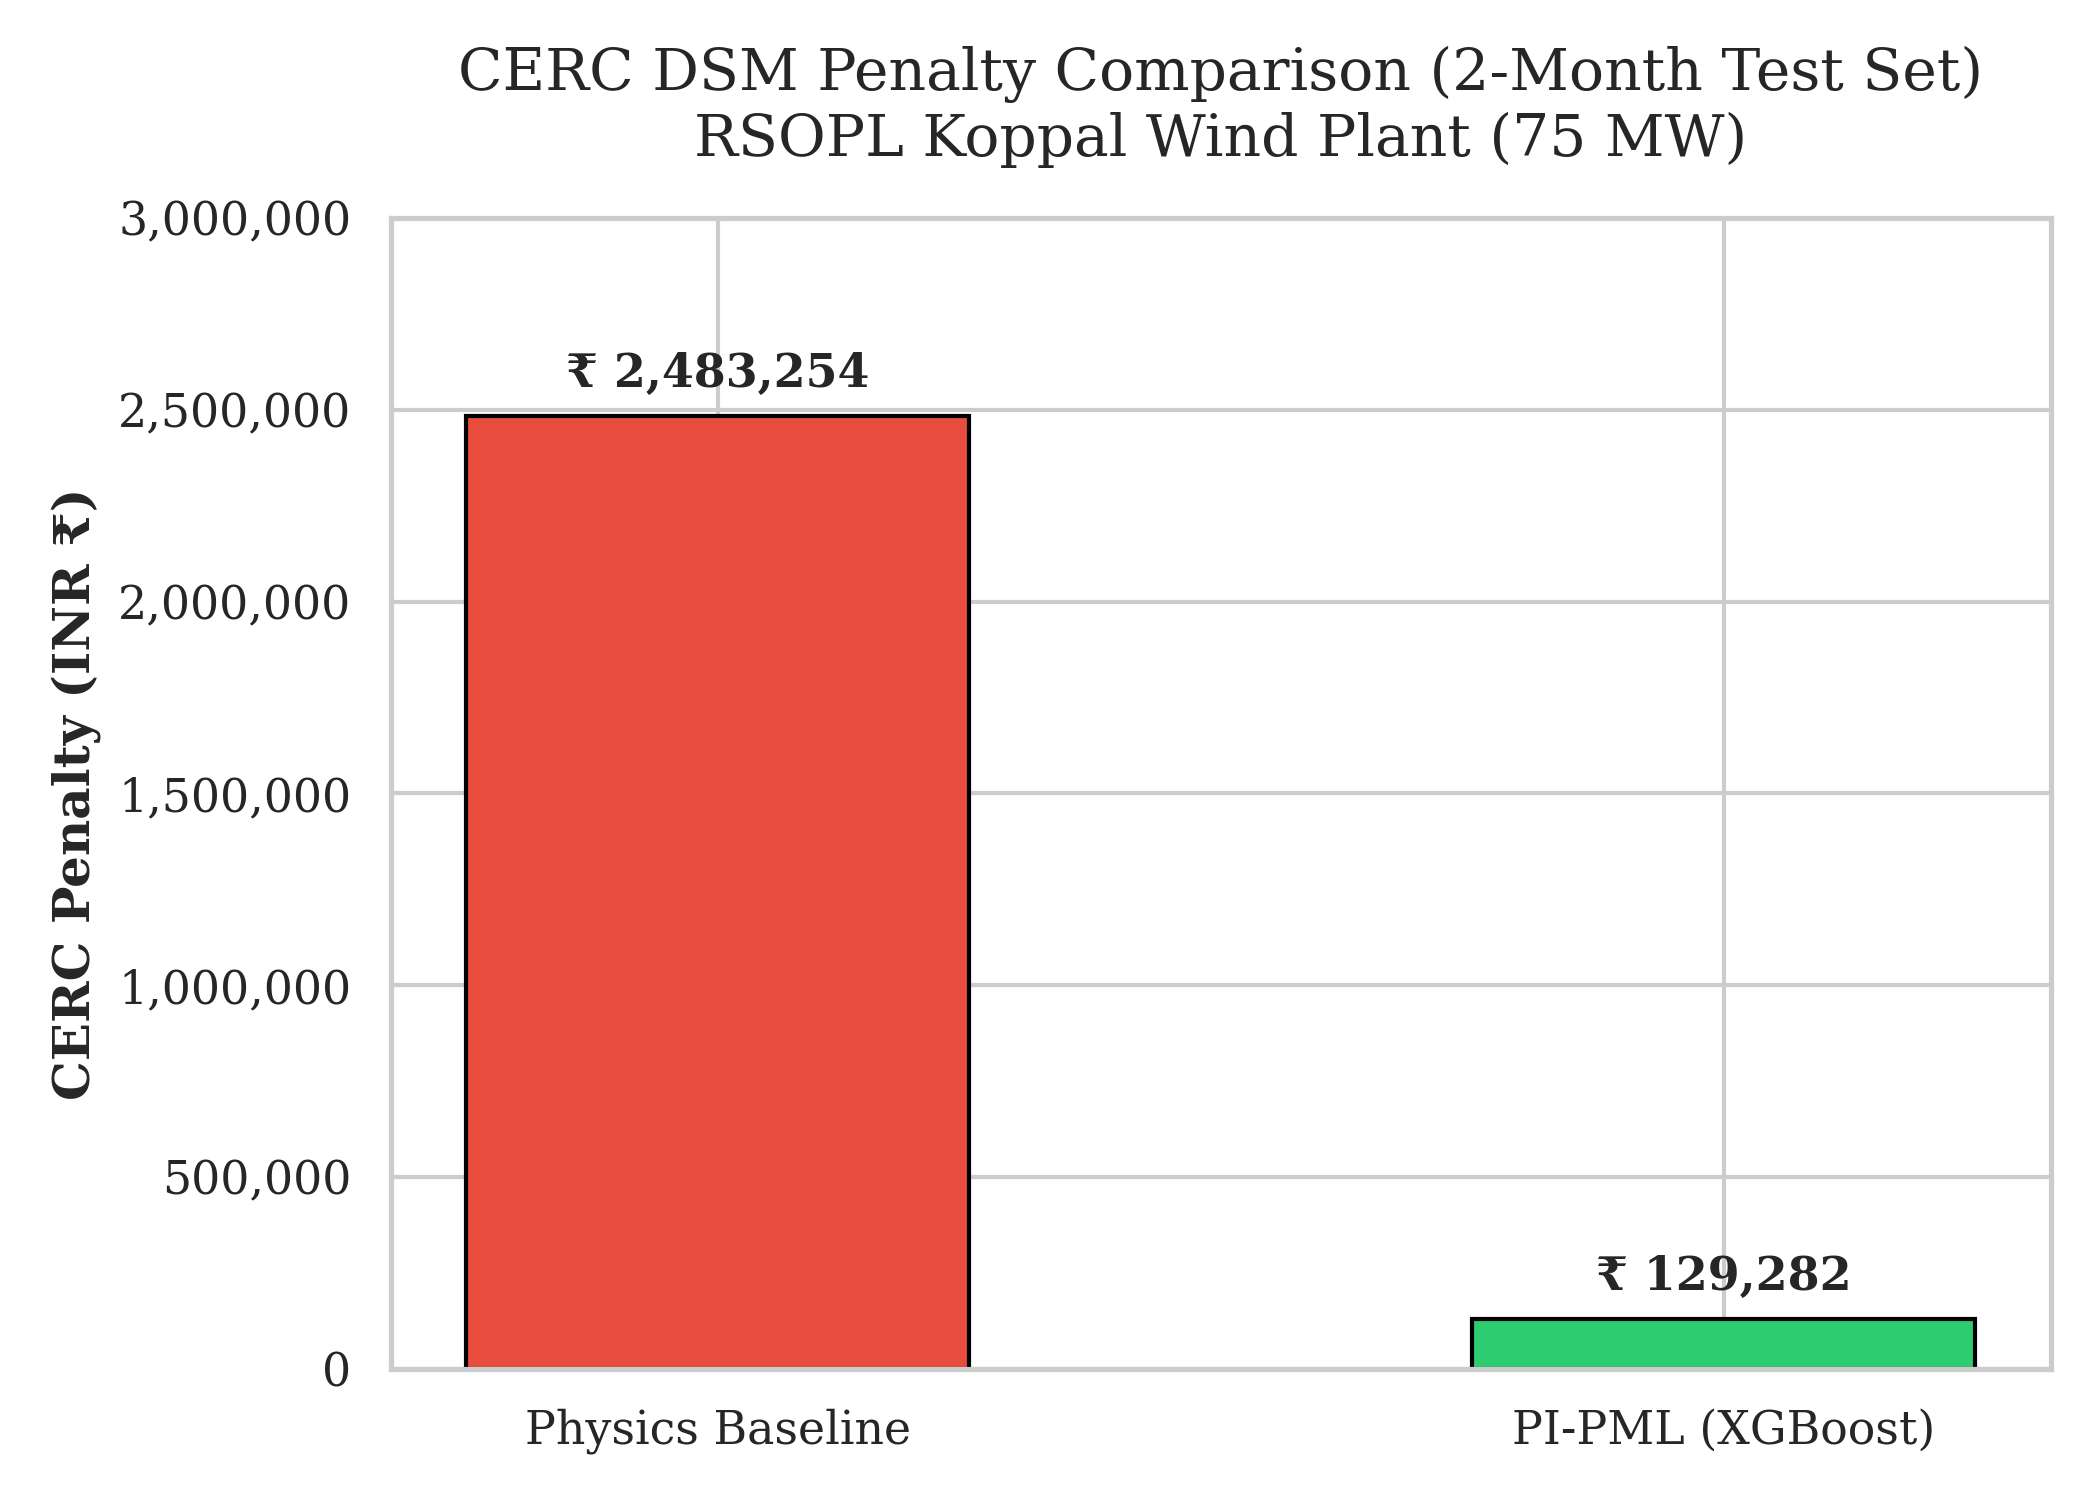
\includegraphics[width=\textwidth]{../penalty_chart.png}
      \\[4pt]
      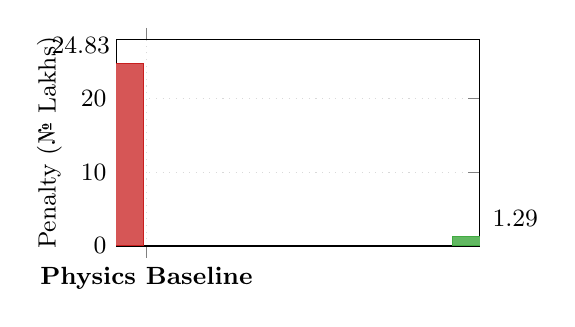
\begin{tikzpicture}
        \begin{axis}[
          ybar, bar width=1.6cm,
          width=6.2cm, height=4.2cm,
          symbolic x coords={Physics Baseline, PI-PML (XGBoost)},
          xtick=data,
          x tick label style={font=\small\bfseries},
          ymin=0, ymax=28,
          ylabel={\small Penalty (\rupee{} Lakhs)},
          ylabel style={font=\small},
          nodes near coords, nodes near coords align=vertical,
          nodes near coords style={font=\small\bfseries},
          grid=major, grid style={dotted,gray!30},
          tick label style={font=\small},
        ]
          \addplot[fill=DSMred!75,draw=DSMred]
            coordinates {(Physics Baseline,24.83)};
          \addplot[fill=MLgreen!75,draw=MLgreen!90]
            coordinates {(PI-PML (XGBoost),1.29)};
        \end{axis}
      \end{tikzpicture}
  \end{columns}
\end{frame}

%────────────────────────────────────────────────────────────────────────────
% SLIDE 10 — LITERATURE REVIEW
%────────────────────────────────────────────────────────────────────────────
\begin{frame}{Literature Review — Theoretical Foundations}
  \begin{center}
    \small\renewcommand{\arraystretch}{1.4}
    \begin{tabularx}{\textwidth}{@{}lXl@{}}
      \toprule
      \textbf{Project Component} & \textbf{Research Area} & \textbf{Key Reference} \\
      \midrule
      \rowcolor{WindBlue!8}
      PI-PML Double-Engine & Theory-Guided Data Science & Karpatne et al.\ (2017) \\
      Residual XGBoost & Hybrid Grey-Box Modelling & Zhao et al.\ (2016) \\
      \rowcolor{WindBlue!8}
      CERC Penalty Logic & Power Systems Economics & Singh et al.\ (2020) \\
      Moist Air Density & Turbine Aerodynamics & Rogers et al.\ (2014) \\
      \rowcolor{WindBlue!8}
      PCHIP + XGBoost & Temporal Signal Processing & Chen et al.\ (2018) \\
      windpowerlib & Open-Source Turbine Modelling & Haas et al.\ (2019) \\
      \rowcolor{WindBlue!8}
      MLflow Lifecycle & ML Operations & Zaharia et al.\ (2018) \\
      \bottomrule
    \end{tabularx}
  \end{center}

  \vspace{4pt}
  \begin{columns}[T]
    \column{0.49\textwidth}
      \begin{block}{TGDS — Karpatne (2017)}
        \small Purely data-driven models violate physical constraints and fail to generalise. \emphblue{Anchoring with physics} ensures plausible predictions — validates the Double-Engine design.
      \end{block}
    \column{0.49\textwidth}
      \begin{block}{Residual Learning — Zhao (2016)}
        \small Training ML on physics residuals outperforms end-to-end ML because residuals have \emphgreen{smaller dynamic range} and are more stationary.
      \end{block}
  \end{columns}
\end{frame}

%────────────────────────────────────────────────────────────────────────────
% SLIDE 11 — CONCLUSION & FUTURE WORK
%────────────────────────────────────────────────────────────────────────────
\begin{frame}{Conclusion \& Future Work}
  \begin{columns}[T]
    \column{0.52\textwidth}
      \begin{tcolorbox}[greenbox, title={\faTrophy\; Key Achievements}]
        \begin{itemize}[leftmargin=1em, itemsep=4pt, font=\small]
          \item \emphgreen{\faCheck} Double-Engine PI-PML pipeline, end-to-end
          \item \emphgreen{\faCheck} GFS spatial (25~km$\to$1~km) \& temporal (3-hr$\to$15-min) downscaling
          \item \emphgreen{\faCheck} Full CERC DSM 3-zone penalty simulator
          \item \emphgreen{\faCheck} MLflow Champion-Challenger lifecycle
          \item \emphgreen{\faCheck} \textbf{71.2\% MAE reduction} on held-out test
          \item \emphgreen{\faCheck} \textbf{94.8\% penalty reduction} (\rupee{}24.8L $\to$ \rupee{}1.3L)
          \item \emphgreen{\faCheck} \emphred{\rupee{}1.41 Crores} projected annual savings
          \item \emphgreen{\faCheck} Live Glassmorphism operator dashboard
        \end{itemize}
      \end{tcolorbox}

    \column{0.46\textwidth}
      \begin{block}{Current Limitations}
        \begin{itemize}[leftmargin=1em, itemsep=3pt, font=\small]
          \item Single-plant validation; multi-plant generalisation needed
          \item GFS accuracy degrades beyond 48-hr horizon
          \item Real-time SCADA not yet in production
        \end{itemize}
      \end{block}

      \vspace{6pt}
      \begin{alertblock}{Future Work}
        \begin{itemize}[leftmargin=1em, itemsep=3pt, font=\small]
          \item \emphblue{Multi-plant ensemble} across correlated parks
          \item \emphblue{Quantile XGBoost} — probabilistic intervals
          \item \emphblue{Temporal Fusion Transformers (TFT)}
          \item \emphblue{Live SCADA} real-time data ingestion
          \item \emphblue{DISCOM intra-state} regulatory support
        \end{itemize}
      \end{alertblock}
  \end{columns}
\end{frame}

%────────────────────────────────────────────────────────────────────────────
% SLIDE 12 — THANK YOU
%────────────────────────────────────────────────────────────────────────────
{
\setbeamercolor{background canvas}{bg=IIITblue}
\begin{frame}[plain]
  \centering
  \vspace{1.6cm}
  {\color{white}\Huge\bfseries Thank You}\\[10pt]
  {\color{MLflow}\large Questions \& Discussion}\\[18pt]
  {\color{white!55}\rule{0.5\textwidth}{0.4pt}}\\[12pt]
  \begin{columns}[c]
    \column{0.5\textwidth}
      \centering
      {\color{white!80}\small\textbf{Tapas Barman} \;|\; MSD24021}\\[3pt]
      {\color{white!55}\small\faEnvelope\; tapasbarman.iiitl@iiitl.ac.in}
    \column{0.5\textwidth}
      \centering
      {\color{white!75}\small\textbf{Dr.\ Sirsendu Sekhar Barman}}\\[2pt]
      {\color{white!55}\small Dept.\ of Mathematics, IIIT Lucknow}
  \end{columns}
  \vfill
  
\includegraphics[width=0.12\textwidth]{../iiitl_logo.png}\\[4pt]
  {\color{white!35}\tiny \textcopyright\ IIIT Lucknow, 2026}
\end{frame}
}

\end{document}
